%% This document is created by 
%%  Dr. Putu Harry Gunawan
%% Template untuk Proposal TA 1 dan TA
%% Template ini digunakan untuk penulisan proposal TA 1 atau TA Fakultas Informatika, Telkom University.
%%  New Update 28 Pebruari 2017 : Bookmarks pdf, Pembimbing hanya satu

\documentclass[a4paper,12pt,oneside]{book}
\usepackage[table]{xcolor}
\usepackage{caption}
\usepackage{capt-of}
\usepackage{anysize}
\usepackage{nameref}

\usepackage{pgfplotstable}
\usepackage{pgfplots}
\pgfplotsset{compat=1.16}
% \usepgfplotslibrary{external} 
% \tikzexternalize

\usepackage{placeins}
\usepackage[utf8]{inputenc}
\usepackage{sectsty}
\usepackage{graphicx}
\graphicspath{./images/}
\usepackage{epstopdf}
\usepackage{algorithm}
\usepackage{algpseudocode}
\usepackage{array}
\usepackage{amsmath}
\usepackage{amssymb}
\usepackage[bahasa]{babel}
\usepackage{indentfirst} %Spasi untuk paragraf pertama
\usepackage{geometry}
\usepackage{multirow}% http://ctan.org/pkg/multirow
\usepackage{hhline}% http://ctan.org/pkg/hhline
\marginsize{4cm}{3cm}{3cm}{3cm} %{left}{right}{top}{bottom}
\usepackage[compact]{titlesec} 
\usepackage{etoolbox}
\usepackage{natbib} %for Harvard syle
\usepackage[bookmarks,hypertexnames=false,debug]{hyperref}
%\usepackage[pageanchor]{hyperref}
\usepackage{bookmark}


\makeatletter
\patchcmd{\ttlh@hang}{\parindent\z@}{\parindent\z@\leavevmode}{}{}
\patchcmd{\ttlh@hang}{\noindent}{}{}{}
\makeatother

\chapterfont{\centering}
\newcommand{\bigsize}{\fontsize{16pt}{14pt}\selectfont}
\chapterfont{\centering\bigsize\bfseries}
\sectionfont{\large\bfseries}
\usepackage{tikz}
\usetikzlibrary{shapes.geometric, arrows}
%\renewcommand{\chaptertitle}{BAB}
\renewcommand{\thechapter}{\Roman{chapter}}
\renewcommand\thesection{\arabic{chapter}.\arabic{section}}
\renewcommand\thesubsection{\thesection.\arabic{subsection}}
\renewcommand{\theequation}{\arabic{chapter}.\arabic{equation}}
\renewcommand{\thefigure}{\arabic{chapter}.\arabic{figure}}
\renewcommand{\thetable}{\arabic{chapter}.\arabic{table}}

\renewcommand\bibname{Daftar Pustaka}
\addto{\captionsbahasa}{\renewcommand{\bibname}{Daftar Pustaka}}
\usepackage{fancyhdr}
\pagestyle{fancy}
\lhead{}
\chead{}
\rhead{}
\lfoot{}
\cfoot{\thepage}
\rfoot{}
\renewcommand{\headrulewidth}{0pt}

\makeatletter

%%%%%%%%%%%%%%%%%%%%%%%%%%%%%%%%%%%%%%%%%%%%%%%%%%%%%%%%%%%%
%
%  Berikut adalah data-data yang wajib diisi oleh mahasiswa
%
%%%%%%%%%%%%%%%%%%%%%%%%%%%%%%%%%%%%%%%%%%%%%%%%%%%%%%%%%%%%

\title{Aplikasi Neural Network Untuk Prediksi Runup Gelombang Pada Terumbu Karang}\let\Title\@title   %Judul dalam bahasa Indonesia

\newcommand{\EngTitle}{Neural Network Application For Predicting Wave Runup On Fringing Reef}  %Judul dalam bahasa Inggris

\author{Yana Agun Siswanto}  \let\Author\@author  %Nama mhs
\newcommand{\NIM}{1301150773}
\newcommand{\Prodi}{Teknik Informatika}
\newcommand{\KK}{Modelling Computational Experiment} %UNTUK TA
\newcommand{\Gelar}{Sains Komputasi} % UNTUK TA
\date{2018}           \let\Date\@date %Masukkan hanya tahun saja
\newcommand{\Tanggal}{22} % Tanggal Pengesahan
\newcommand{\Bulan}{Agustus} % Bulan Pengesahan
\newcommand{\PembimbingSatu}{Dr. Didit Aditya, S.Si, M.Si}
\newcommand{\NIPPembimbingSatu}{16830005}
\newcommand{\PembimbingDua}{Dr. Putu Harry Gunawan, S.Si., M.Si., M.Sc.}
\newcommand{\NIPPembimbingDua}{16860043}
\newcommand{\Kaprodi}{}
\newcommand{\NIPKaprodi}{95650581-1}
\newif\ifPembimbingHanyaSatu

%%%% WARNING kode berikut ini diaktifkan Jika pembimbing hanya satu %%%%

%\PembimbingHanyaSatutrue

%%%%%%%%%%%%%%%%%%%%%%%%%%%%%%%%%%%%%%%%%%%%%%%%%%%%%%%%%%%%%%%%%%

\makeatother
\linespread{1}


\begin{document}
%%%%%%%%%%%%%%%%%%%%%%%%%%%%%%%%%%%%%%%%%%%%%%%%%%%%%%%%%%
% Dimulai dengan cover, lembar persetujuan, Abstrak, dll
%%%%%%%%%%%%%%%%%%%%%%%%%%%%%%%%%%%%%%%%%%%%%%%%%%%%%%%%%%%
\pagenumbering{roman} 
\begin{titlepage}
\thispagestyle{empty}
%\vspace*{0.7cm}
\pdfbookmark{Cover}{ }
{\centering
\large
{\bigsize\bf \Title}\\
\vspace{ 2cm}
\rm
\textbf{Proposal Tugas Akhir}\\
\vspace{0.5 cm}
\textbf{Kelas TA 1}\\
\vspace{0.5 cm}
\textbf{\Author}\\ \textbf{NIM: \NIM}\\ 

\vspace{1.5 cm}

\begin{figure}[h]
{\centering {
\includegraphics[scale=0.17]{Tel-U-Logo}}\par}
\end{figure}

\vspace{2 cm}
{\bigsize\textbf{Program Studi Sarjana \Prodi}\\
\vspace{0.5 cm}
\textbf{Fakultas Informatika}\\
\vspace{0.5 cm}
\textbf{Universitas Telkom}\\
\vspace{0.5 cm}
\textbf{Bandung}\\
\vspace{0.5 cm}
\textbf{\Date}\\}
}
\pagebreak
\thispagestyle{empty}
\pdfbookmark{Lembar Persetujuan}{ }
{\centering
\textbf{\large Lembar Persetujuan}\\
\vspace{0.5cm}
\textbf{\Title}\\
\vspace{0.5cm}
\textbf{\textit{\EngTitle}}\\
\vspace{0.5cm}
\textbf{\Author}\\
\textbf{NIM: \NIM}\\
\vspace{1cm}


{ Proposal ini diajukan sebagai usulan pembuatan tugas akhir pada\\ Program Studi Sarjana \Prodi\\ Fakultas Informatika Universitas Telkom}\\

\vspace{0.5cm}

{Bandung, \Tanggal\quad \Bulan \quad \Date}\\
{Menyetujui}\\

\vspace{0.5cm}
      \ifPembimbingHanyaSatu
             \begin{center}
            Calon Pembimbing 1
            \end{center}
       \else
          \begin{center}
              \begin{tabular}{  m{8cm}  m{8cm} }
              Calon Pembimbing 1 & Calon Pembimbing 2
              \end{tabular}
           \end{center}
      \fi
\begin{center}
\vspace{2cm}
\ifPembimbingHanyaSatu
     \underline{\PembimbingSatu} \\ 
      NIP: \NIPPembimbingSatu
\else
\begin{tabular}{  m{8cm}  m{8cm} }
\underline{\PembimbingSatu} & \underline{\PembimbingDua} \\ 
NIP: \NIPPembimbingSatu & NIP: \NIPPembimbingDua
\end{tabular}
\fi
\end{center}
\vspace{0.5cm}

}
\pagebreak
\end{titlepage}
\phantomsection
\addcontentsline{toc}{chapter}{Abstrak}
%\pdfbookmark{\abstractname}{Abstrak Indonesia}
\chapter*{Abstrak}
Sebagian besar dari permukaan bumi merupakan permukaan air. Dampak yang air berikan kepada struktur geografis daratan di bumi sangatlah besar. Penyebabnya adalah ketika air memasuki daratan sebagai akibat adanya energi luar yang mempengaruhi kondisi stabil air saat itu. Dengan memasang sensor ketinggian gelombang, arah gelombang, serta kecepatan angin, kita dapat memprediksi seberapa jauh dan tinggi air memasuki daratan. 
\vspace{0.5 cm}
\begin{flushleft}
{\textbf{Kata Kunci:} Terumbu karang, Gelombang Air Laut.}
\end{flushleft}
\cleardoublepage
\phantomsection
\addcontentsline{toc}{chapter}{Daftar Isi}
%\pdfbookmark{\contentsname}{Contents}
\tableofcontents

%%%%%%%%%%%%%%%%%%%%%%%%%%%%%%%%%%%%%%%%%%%%%%%%%
% Bab bab penulisan
%%%%%%%%%%%%%%%%%%%%%%%%%%%%%%%%%%%%%%%%%%%%%%%%
\cleardoublepage
\pagenumbering{arabic}
\chapter{Pendahuluan}
\section{Latar Belakang}

Terumbu karang adalah ekosistem bawah laut yang terbentuk dari sekumpulan karang. Selain berfungsi sebagai ekosistem di bawah laut, terumbu karang juga berfungsi sebagai pemecah gelombang. Sebagian besar kepulauan di wilayah pasific di kelilingi oleh terumbu karang yang tumbuh di laut dangkal yang dekat dengan pantai \cite{DemirbilekBoussinesq}.

\begin{figure}[htp]
    \begin{center}
        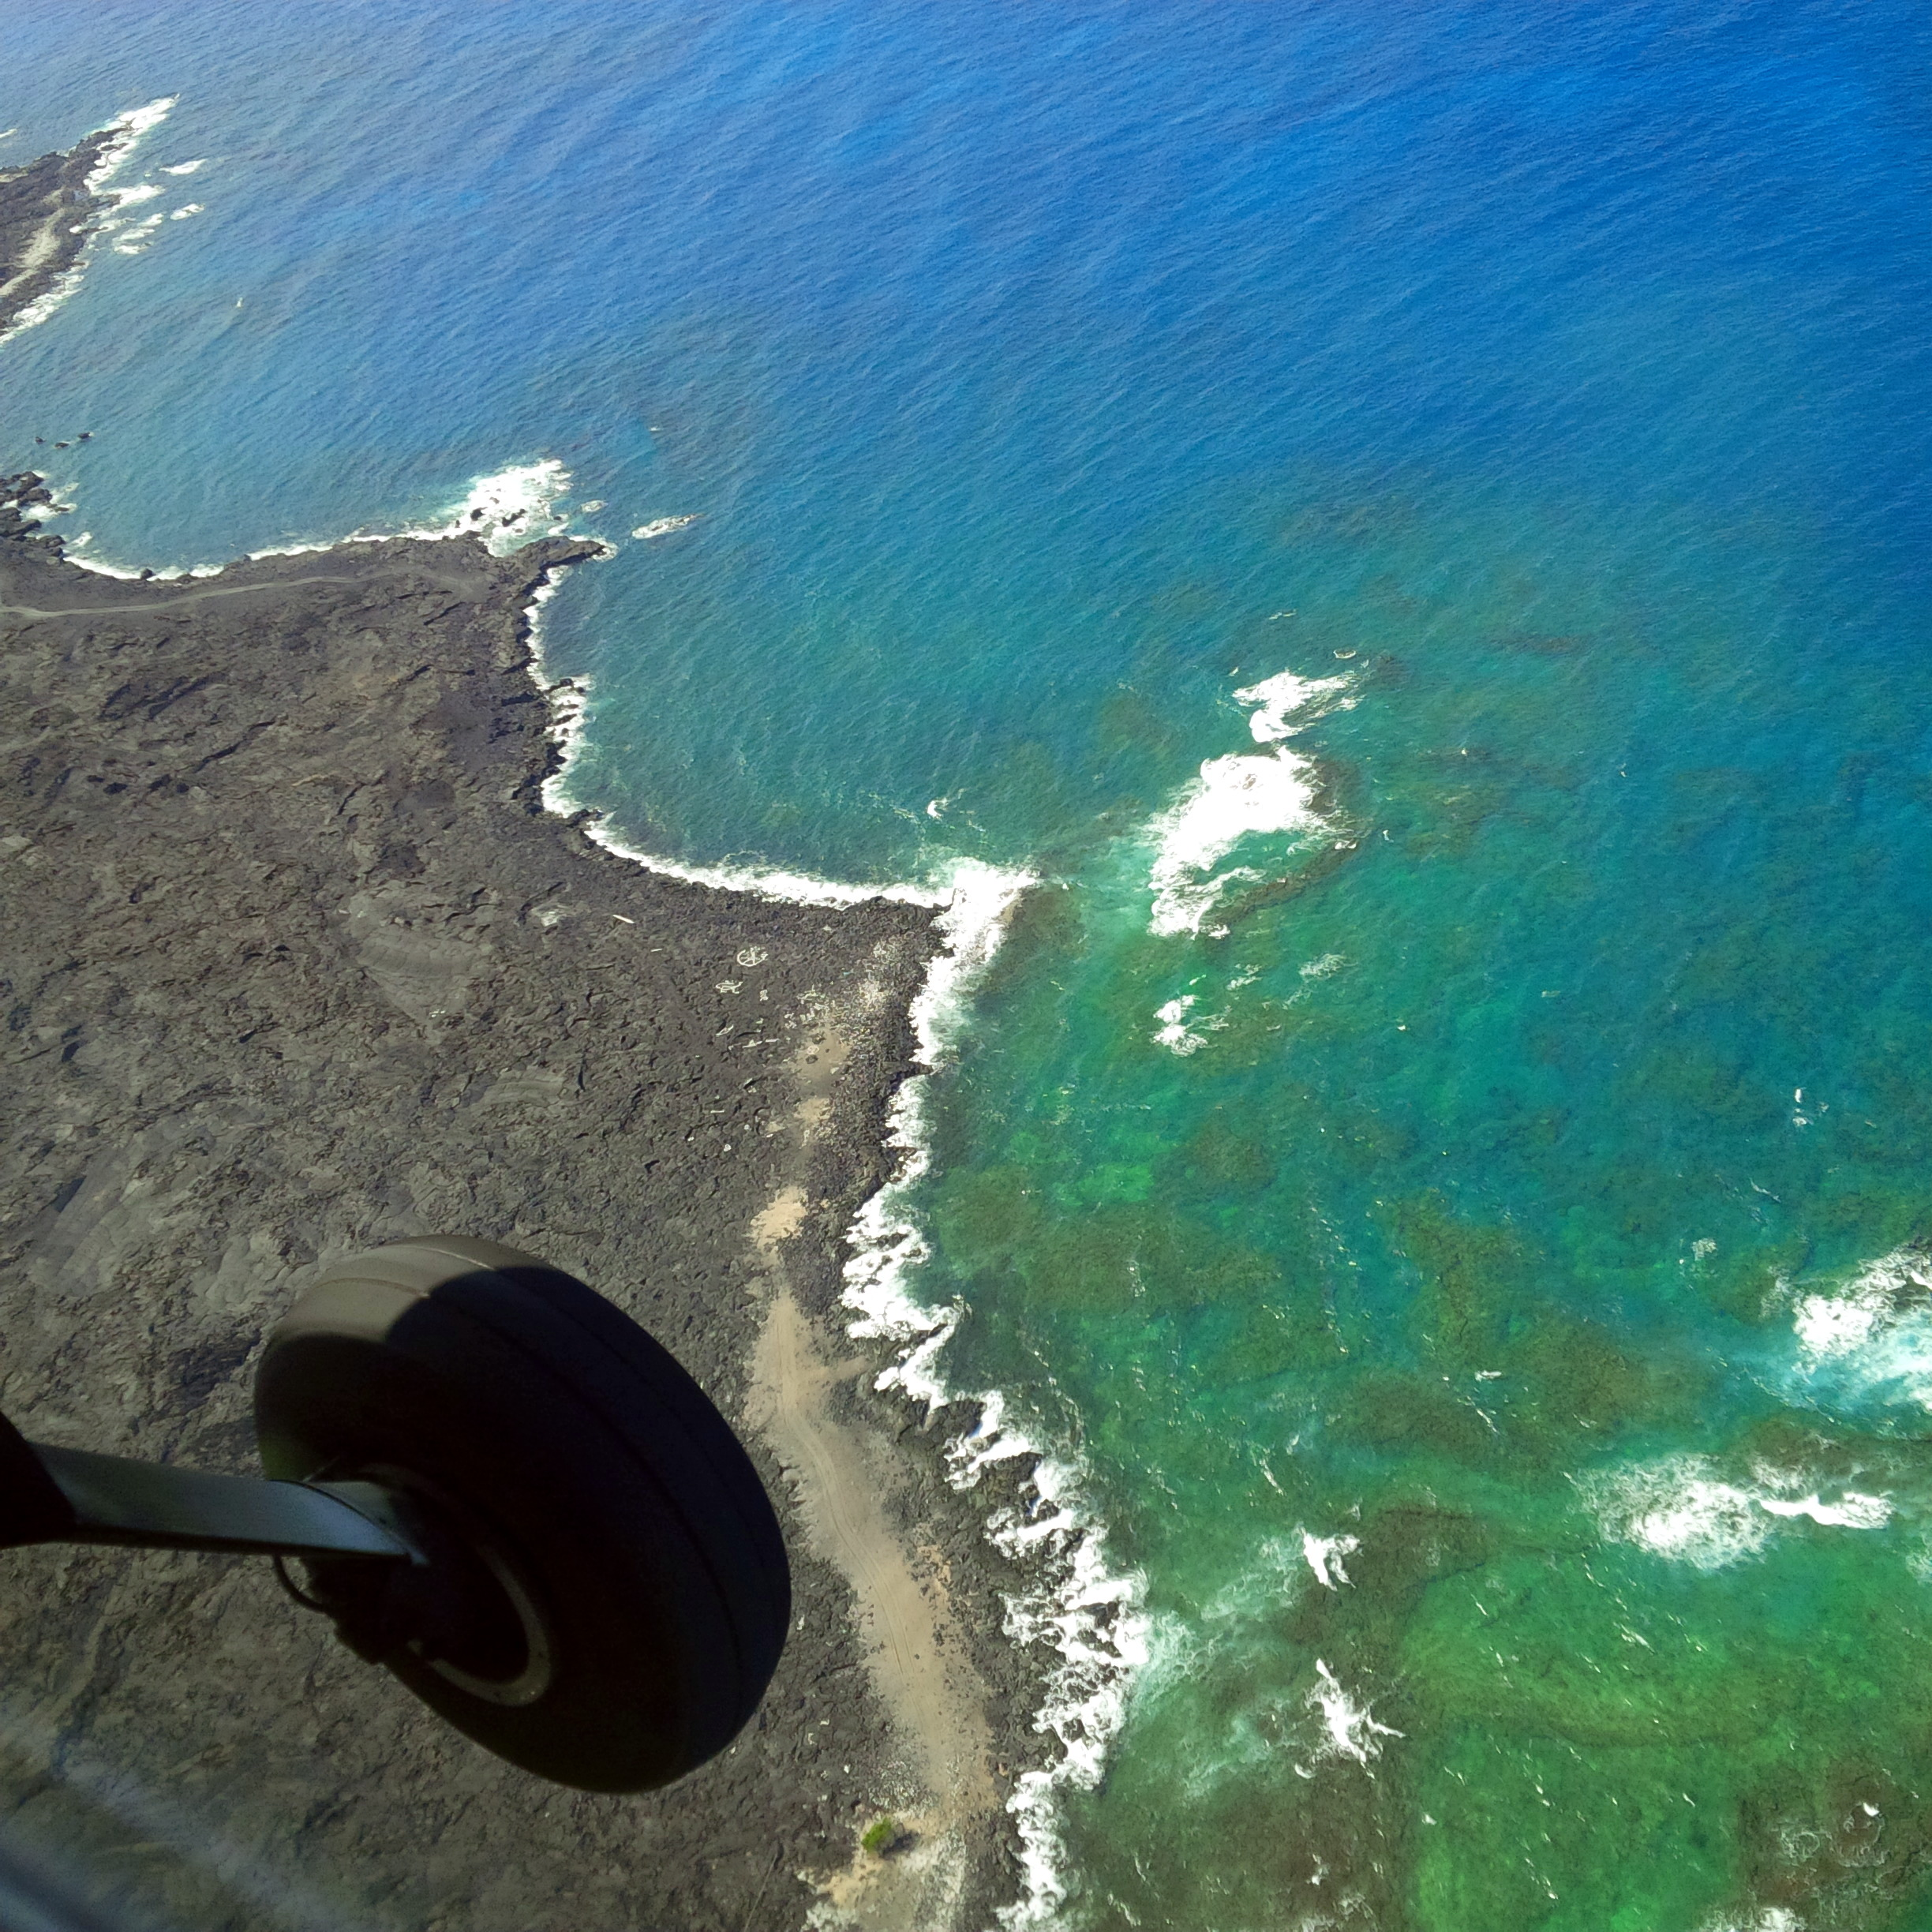
\includegraphics[scale=0.1]{./images/hawai_coral.jpg}
    \end{center}
    \caption{Terumbu Karang di tepi pantai di sekitar Hawai.}
\end{figure}

Gelombang yang melewati terumbu karang akan teredam kecepatannya \cite{DemirbilekReport}. Hal ini akan mempengaruhi naiknya gelombang ke daratan di atas batas normal, atau dalam literatur lain disebut \emph{runup} gelombang \cite{nielsen1991wave}. Teredamnya kecepatan gelombang disebabkan oleh bertumbukannya dasar gelombang dengan karang. Dalam beberapa kasus, hal ini menyebabkan pecahnya gelombang \cite{DemirbilekReport}

Namun efektifitas dari terumbu karang dalam meredam gelombang masih menjadi perdebatan para peneliti. Yang selama ini dilakukan dalam mempelajari redaman dari terumbu karang adalah eksperimen di laboratorium. Seperti yang dilakukan Yau et al (2012)\cite{YAO201230}, dia mengerjakannya dengan menggunakan model \emph{Boussinesq} 1 dimensi untuk memodelkan transformasi gelombang saat melewati terumbu karang.  Namun cara mempelajari ini tergolong mahal dan membutuhkan pemodelan matematika yang dalam untuk memodelkan pecahnya gelombang.

Selama ini metode yang ada untuk memprediksi tinggi gelombang \emph{runup} pada terumbu karang masih tergolong baru. Metodenya sendiri terbagi menjadi 2. Metode yang pertama dilakukan dengan pendekatan klasik, dan di lakukan secara analitis. Yakni dengan melakukan eksperimen dan observasi, lalu di cari model matematika yang tepat. Model yang demikian sulit untuk dikembangkan dan beradaptasi dengan kondisi lingkungan yang berbeda. Prediksi yang didapat dari model yang demikian pun masih belum sempurna \cite{DemirbilekBoussinesq}. Sedangkan metode yang kedua dilakukan dengan pendekatan \emph{soft computing}.

Pada TA ini kami menggunakan Pembelajaran Mesin untuk memprediksi \emph{runup} gelombang. Metode yang digunakan disini adalah \emph{supervised learning}, dengan menggunakan data dari Demirbilek et al (2007)\cite{DemirbilekReport}. Dari data hasil \emph{training} dan \emph{testing} dengan konfigurasi neural network. Diharapakan mendapatkan model dengan akurasi yang tinggi. Sehingga efisiensi dari terumbu karang dalam memecahkan gelombang dapat dipelajari dengan baik.

\section{Perumusan Masalah}
Rumusan masalah yang ingin yang angkat pada TA ini adalah
\begin{enumerate}
    \item Bagaimana melakukan pemodelan supervised learning dengan data eksperimen yang dilakukan di laboratorium?
    \item Bagaimana akurasi dari model prediksi runup gelombang yang telah dibuat?
    \item Seberapa efisien terumbu karang dalam meredam gelombang?
\end{enumerate}
\section{Tujuan}
Berikut adalah tujuan yang ingin dicapai pada penulisan proposal/TA.
\begin{enumerate}
    \item Memodelkan data hasil eksperimen di laboratorium menggunakan \emph{supervised learning}
    \item Mengetahui akurasi Artificial Neural Network untuk prediksi \emph{runup} gelombang pada terumbu karang.
    \item Mengetahui efisiensi dari terumbu karang dalam meredam gelombang.
\end{enumerate}
\section{Batasan Masalah}
Untuk memastikan hasil yang cukup akurat. Lingkupan masalah diperkecil menjadi:
\begin{enumerate}
    \item Data berasal dari eksperimen pada laboratorium dinamika oleh Demerbilek (2007).
    \item Metode yang digunakan pada eksperimen ini adalah Artificial Neural Network.
\end{enumerate}
\section{Rencana Kegiatan}
Rencana kegiatan yang akan saya lakukan adalah sebagai berikut:
\begin{itemize}
    \item Studi literatur: Pengumpulan informasi dan referensi.
    \item Penentuan Topik
    \item Analisis dan Perancangan Sistem
    \item Implementasi Sistem
    \item Analisa Hasil Implementasi
    \item Penulisan Laporan
\end{itemize}
\section{Jadwal Kegiatan}

Laporan proposal ini akan dijadwalkan sesuai dengan tabel berikut:

 
\begin{table}[h!]
  \centering
    \caption{Jadwal kegiatan proposal tugas akhir}
  \label{Novella}
  \begin{tabular}{|c|m{2.5cm}|m{0.01cm}|m{0.01cm}|m{0.01cm}|m{0.01cm}|m{0.01cm}|m{0.01cm}|m{0.01cm}|m{0.01cm}|m{0.01cm}|m{0.01cm}|m{0.01cm}|m{0.01cm}|m{0.01cm}|m{0.01cm}|m{0.01cm}|m{0.01cm}|m{0.01cm}|m{0.01cm}|m{0.01cm}|m{0.01cm}|m{0.01cm}|m{0.01cm}|m{0.01cm}|m{0.01cm}|}
    \hline
    \multirow{2}{*}{\textbf{No}} & \multirow{2}{*}{\textbf{Kegiatan}} & \multicolumn{24}{|c|}{\textbf{Bulan ke-}} \\
    \hhline{~~------------------------}
    {} & {} & \multicolumn{4}{|c|}{\textbf{1}} & \multicolumn{4}{|c|}{\textbf{2}} & \multicolumn{4}{|c|}{\textbf{3}} & \multicolumn{4}{|c|}{\textbf{4}} & \multicolumn{4}{|c|}{\textbf{5}} & \multicolumn{4}{|c|}{\textbf{6}}\\
    \hline
    1 & Studi Literatur & \cellcolor{blue!25} & \cellcolor{blue!25} & \cellcolor{blue!25} & \cellcolor{blue!25}& \cellcolor{blue!25} & \cellcolor{blue!25} & \cellcolor{blue!25} & \cellcolor{blue!25}& \cellcolor{blue!25} & \cellcolor{blue!25} & \cellcolor{blue!25} & \cellcolor{blue!25}& \cellcolor{blue!25} & \cellcolor{blue!25} & \cellcolor{blue!25} & \cellcolor{blue!25}& \cellcolor{blue!25} & \cellcolor{blue!25} & \cellcolor{blue!25} & \cellcolor{blue!25}& \cellcolor{blue!25} & \cellcolor{blue!25} & \cellcolor{blue!25} & \cellcolor{blue!25}\\
    \hline
    2 & Analisis dan Perancangan Sistem &  {} & {} & {} & {}  & \cellcolor{blue!25} & \cellcolor{blue!25} & \cellcolor{blue!25} & \cellcolor{blue!25} & \cellcolor{blue!25} & \cellcolor{blue!25} & \cellcolor{blue!25} & \cellcolor{blue!25} & {} & {} & {} & {}& {} & {} & {} & {}& {} & {} & {} & {}\\
    \hline
    3 & Implementasi Sistem &  {} & {} & {} & {} & {} & {} & {} & {}& \cellcolor{blue!25} & \cellcolor{blue!25} & \cellcolor{blue!25} & \cellcolor{blue!25} & \cellcolor{blue!25} & \cellcolor{blue!25} & \cellcolor{blue!25} & \cellcolor{blue!25} & {} & {} & {} & {}& {} & {} & {} & {}\\
    \hline
    4 & Analisa Hasil Implementasi &  {} & {} & {} & {} & {} & {} & {} & {}& {} & {} & {} & {} & \cellcolor{blue!25} & \cellcolor{blue!25} & \cellcolor{blue!25} & \cellcolor{blue!25} & \cellcolor{blue!25} & \cellcolor{blue!25} & \cellcolor{blue!25} & \cellcolor{blue!25} & {} & {} & {} & {}\\
    \hline
    5 & Penulisan Laporan & {} & {} & {} & {} & \cellcolor{blue!25} & \cellcolor{blue!25} & \cellcolor{blue!25} & \cellcolor{blue!25}& \cellcolor{blue!25} & \cellcolor{blue!25} & \cellcolor{blue!25} & \cellcolor{blue!25}& \cellcolor{blue!25} & \cellcolor{blue!25} & \cellcolor{blue!25} & \cellcolor{blue!25}& \cellcolor{blue!25} & \cellcolor{blue!25} & \cellcolor{blue!25} & \cellcolor{blue!25}& \cellcolor{blue!25} & \cellcolor{blue!25} & \cellcolor{blue!25} & \cellcolor{blue!25}\\
    \hline
  \end{tabular}
\end{table}


%
\chapter{Kajian Pustaka}

    Pembelajaran mesin sudah banyak dipakai di berbagai bidang keilmuan. Mulai dari Pemrosesan Citra seperti yang di lakukan oleh Lawrence et al (2007)\cite{lawrence1997face}. Beliau menggunakan \emph{neural network} dengan tipe \emph{Convolutional Neural Network} untuk mendeteksi wajah. Van Gent et al (2007) \cite{van2007neural}, beliau menggunakan \emph{Neural Network} untuk menganalisa \emph{overtopping} gelombang pada struktur di wilayah pantai. Yau et al (2012)\cite{YAO201230}, dia mengerjakannya dengan menggunakan model \emph{Boussinesq} 1 dimensi untuk memodelkan transformasi gelombang saat melewati terumbu karang Pada bab ini akan dijelaskan model \emph{runup} gelombang pada terumbu karang menggunakan Pembelajaran Mesin.

\section{Runup Gelombang}

    Runup gelombang adalah jarak vertikal maksimum dari kenaikan gelombang pada pantai atau struktur di atas \emph{SWL} \cite{sorensen2005basic}. Pada TA ini, data ovservasi ketinggian \emph{runup} gelombang diukur mulai ketinggian \emph{swl}, hingga maksimum ketinggian air di daratan. Penjelasan lebih lanjut tentang pengambilan data akan dijelaskan pada bagian \nameref{kondisiEksperimen}. Runup gelombang dapat diilustrasikan dengan gambar berikut:

    \begin{figure}
        \begin{center}
            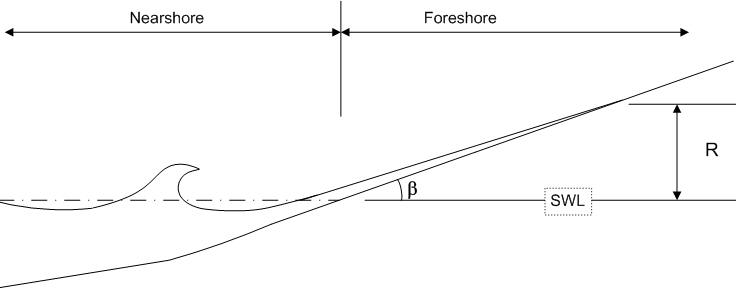
\includegraphics[scale=0.7]{./images/runup_gelombang.jpg}
        \end{center}
        \caption{Ilustrasi \emph{Runup} gelombang oleh Mike Swenson, Coastal Morphology, University of Wisconsin-Madison \cite{MikeSwenson:WaveRunup}. \emph{SWL (Sea Water Level)} adalah ketinggian Air Normal ketika tidak gelombang . Wilayah Pantai (\emph{Foreshore}), dimulai dari titik \emph{SWL} yang berpotongan dengan daratan. Wilayah lautan \emph{Nearshore}, dimulai dari titik \emph{SWL} yang berpotongan dengan air. Ketika titip potong air dengan daratan berada di atas \emph{SWL}, dinamakan \emph{runup}. Ketinggian \emph{runup} dinotasikan dengan $R$.}
    \end{figure}
    \FloatBarrier

\section{Pembelajaran Mesin}
    Pembelajaran mesin adalah bidang studi yang memberikan kemampuan komputer untuk belajar, tanpa harus di program secara khusus \cite{arthur_l_samuel_1959}. Mesin dikatakan belajar dari pengalaman ($E$) terhadap tugas ($T$) dan ukuran kinerja ($P$), jika kinerja pada tugas ($T$), yang di ukur berdasarkan ($P$), berkembang berdasarkan pengalaman ($E$). Dalam TA ini, akan dibuat suatu program yang dapat belajar dari data gelombang hasil observasi ($T$). Lalu dievaluasi hasilnya dengan menggunakan $MSE$ ($P$), sehingga dapat di lihat seberapa besar galatnya. Lalu diperkecil galatnya dengan metode optimasi.

\subsection{Supervised Learning}
    Sebelum data dimasukan ke dalam program, data tersebut diberikan label. Label tersebut bisa berupa \emph{input}, yakni $H$ (\emph{Significant Height} Gelombang), $T$ (\emph{Spectral Peak Periods}), dan $WL$ (\emph{Wave Length}). Dan label untuk \emph{output}. Karna pada TA kali ini, akan digunakan regresi linear. Maka tidak ada label untuk \emph{output}. Parameter \emph{input} yang berpasangan dengan \emph{output} tertentu, selanjutnya dinamakan contoh. Pembelajaran Mesin yang demikian dinamakan \emph{Supervised Learning}. \emph{Supervised Learning} Merupakan bagian dari pembelajaran mesin yang memetaan \emph{input} ke \emph{output} yang berdasar pada contoh pasangan \emph{input} dan \emph{output}\cite{AIPeterNorvig}. 

\subsection{Neural Network}
    Selanjutnya data tersebut dimasukan kedalam suatu sistem untuk belajar. Pada TA ini, sistem yang digunakan untuk pembelajaran adalah \emph{Neural Network}.
    Model \emph{neural network} sederhana di definisikan oleh McCulloch-Pitts \cite{McCulloch1943}. Dimana persamaan memiliki $M$ himpunan \emph{Input} ($I$) (\emph{input neuron}), dan satu \emph{output} ($y$), dengan $y$ merupakan bagian dari $\{0,1\}$. Atau dengan kata lain, $y$ adalah fungsi yang hanya memiliki \emph{output} $0$ dan $1$.
    \begin{equation}
        y = f(z)
    \end{equation}
    dimana
    \begin{equation}
    \label{eq:mcullochNeuralNetwork}
        z = \sum_{i=1}^N I_iW_i
    \end{equation}

    Di TA ini, \emph{output} yang akan dihasilkan tidak terbatas pada $0$ dan $1$. Sehingga di \emph{neuron output}, fungsi aktivasi yang digunakan adalah fungsi aktivasi linear. Model \emph{Neural Network}nya dapat direpresentasikan sebagai berikut:
    \begin{figure}[H]
        \def\layersep{4cm}
        \begin{tikzpicture}[shorten >=1pt,->,draw=black!50, node distance=\layersep]
            \tikzstyle{every pin edge}=[<-,shorten <=1pt]
            \tikzstyle{neuron}=[circle,fill=black!25,minimum size=17pt,inner sep=0pt]
            \tikzstyle{input neuron}=[neuron, fill=green!50];
            \tikzstyle{output neuron}=[neuron, fill=red!50];
            \tikzstyle{hidden neuron}=[neuron, fill=blue!50];
            \tikzstyle{annot} = [text width=4em, text centered]

            % Draw the input layer nodes
            \foreach \name / \y in {1,...,2}
            % This is the same as writing \foreach \name / \y in {1/1,2/2,3/3,4/4}
                \node[input neuron, pin=left:Input \#\y] (I-\name) at (0,-\y) {};

            % Draw the hidden layer nodes
            \foreach \name / \y in {1,...,2}
                \path[yshift=0.0cm]{}
                    node[hidden neuron] (H-\name) at (\layersep,-\y cm) {};

            % Draw the output layer node
            \node[output neuron,pin={[pin edge={->}]right:Output}, right of=H-1] (O) {};

            % Connect every node in the input layer with every node in the
            % hidden layer.
            \foreach \source in {1,...,2}
                \foreach \dest in {1,...,2}
                    \path (I-\source) edge node[midway, right] {$W_{input}$} (H-\dest);

            % Connect every node in the hidden layer with the output layer
            \path (H-1) edge node[midway, right] {$W_{output}$} (O);
            \path (H-2) edge node[midway, right] {$W_{output}$} (O);

            % Annotate the layers
            \node[annot,above of=H-1, node distance=1cm] (hl) {Hidden layer};
            \node[annot,left of=hl] {Input layer};
            \node[annot,right of=hl] {Output layer};
            \label{neuralNetworkRepresentation}
        \end{tikzpicture}
        \caption{Model \emph{Neural Network} dengan 1 \emph{Hidden Layer}.}
    \end{figure}
    Dimana $W$ adalah peubah yang menyatakan berat. Masing masing \emph{input} akan \emph{didot productkan} dengan $W_{input}$ \emph{hidden layer} tertentu untuk menghasilkan nilai pada \emph{hidden layer neuron} tersebut. Selanjutnya, nilai hasil aktivasi di \emph{hidden layer}, akan di \emph{dot productkan} dengan $W_{output}$. Untuk selanjutnya menjadi \emph{output}, yakni prediksi dari runup gelombang.

\subsubsection{Fungsi Aktivasi}
    Fungsi aktivasi digunakan untuk mengubah level aktivasi pada suatu neuron menjadi sebuah sinyal output \cite{KarlicOlgacPerformanceAnalysis}. Pada TA ini, terdapat 2 fungsi aktivasi yang digunakan. Pada hidden layer, digunakan fungsi aktivasi \emph{Rectified Linear Unit (RELU)}. Fungsi aktivasi \emph{RELU} didefinisikan dengan\cite{glorot2011deep}:

    \begin{equation}
        f(x) = max(0, x)
    \end{equation}

    RELU menjadi pilihan karna memiliki performa konvergensi yang lebih baik dibanding sigmoid \cite{Krizhevsky:2012:ICD:2999134.2999257}. Untuk selanjutnya, pada neuron \emph{output}, digunakan fungsi aktivasi linear. Fungsi aktivasi linear didefinisikan dengan\cite{MLBishop}:

    \begin{equation}
        f(x) = x
    \end{equation}

\subsubsection{Estimasi Galat / \emph{Cost / Lost Function}}
    Kalkulasi galat sangat penting untuk menentukan seberapa besar akurasi yang dimiliki model prediksi pada TA ini. Fungsi estimasi galat yang digunakan adalah \emph{Mean Square Error (MSE)}.

    \begin{equation}
        \operatorname{MSE}(\hat{\theta})=\operatorname{E}_{\hat{\theta}}\left[(\hat{\theta}-\theta)^2\right]
    \end{equation}

    \emph{MSE} dipilih sifatnya yang selalu positif. Sifatnya yang selalu positif cocok digunakan pada TA ini karna prediksi pada model yang akan dibuat bisa berupa bilangan negatif.

%
\chapter{Metodologi dan Desain Sistem}
  Metode yang akan digunakan pada TA ini adalah Artificial Neural Network. Data hasil analisa Demirbilek et al (2007) \cite{DemirbilekReport} akan dibagi 2. Yakni 80 persen untuk training, dan 20 persen untuk testing. Masing masing, akan disimpan ke dalam file csv. Sistem akan membaca data training langsung dari file, lalu dimasukannya sebagai input ke dalam algoritma ANN. Setelah training, sistem akan menghasilkan suatu model dengan matriks dengan attribut $W_{input}$ dan $W_{output}$ di dalamnya. Tujuannya adalah mendapatkan suatu model yang cukup baik untuk menghasilkan prediksi yang cukup akurat.

\section{Deskripsi Data}
Data yang akan digunakan dalam aplikasi neural network di TA ini adalah data hasil analisis dari eksperimen yang di lakukan oleh US Army Corps of Engineer pada Agustus - September 2006. Analisa dilakukan oleh Demirbilek et al. dan di tulis dalam laporan yang berjudul \emph{"Laboratory Study of Wind Effect on Runup over Fringing Reefs"}.

\subsection{Kondisi Eksperimen}
\label{kondisiEksperimen}

Eksperimen dibagi menjadi 3 bagian. Eksperimen pertama dilakukan hanya menggunakan variabel gelombang, dengan kecepatan angin 0. Eksperimen kedua, dilakukan hanya menggunakan variabel angin. Selanjutnya eksperimen ketiga adalah gabungan dari perubahan variable gelombang dan variabel angin.

\begin{figure}
  \begin{center}
    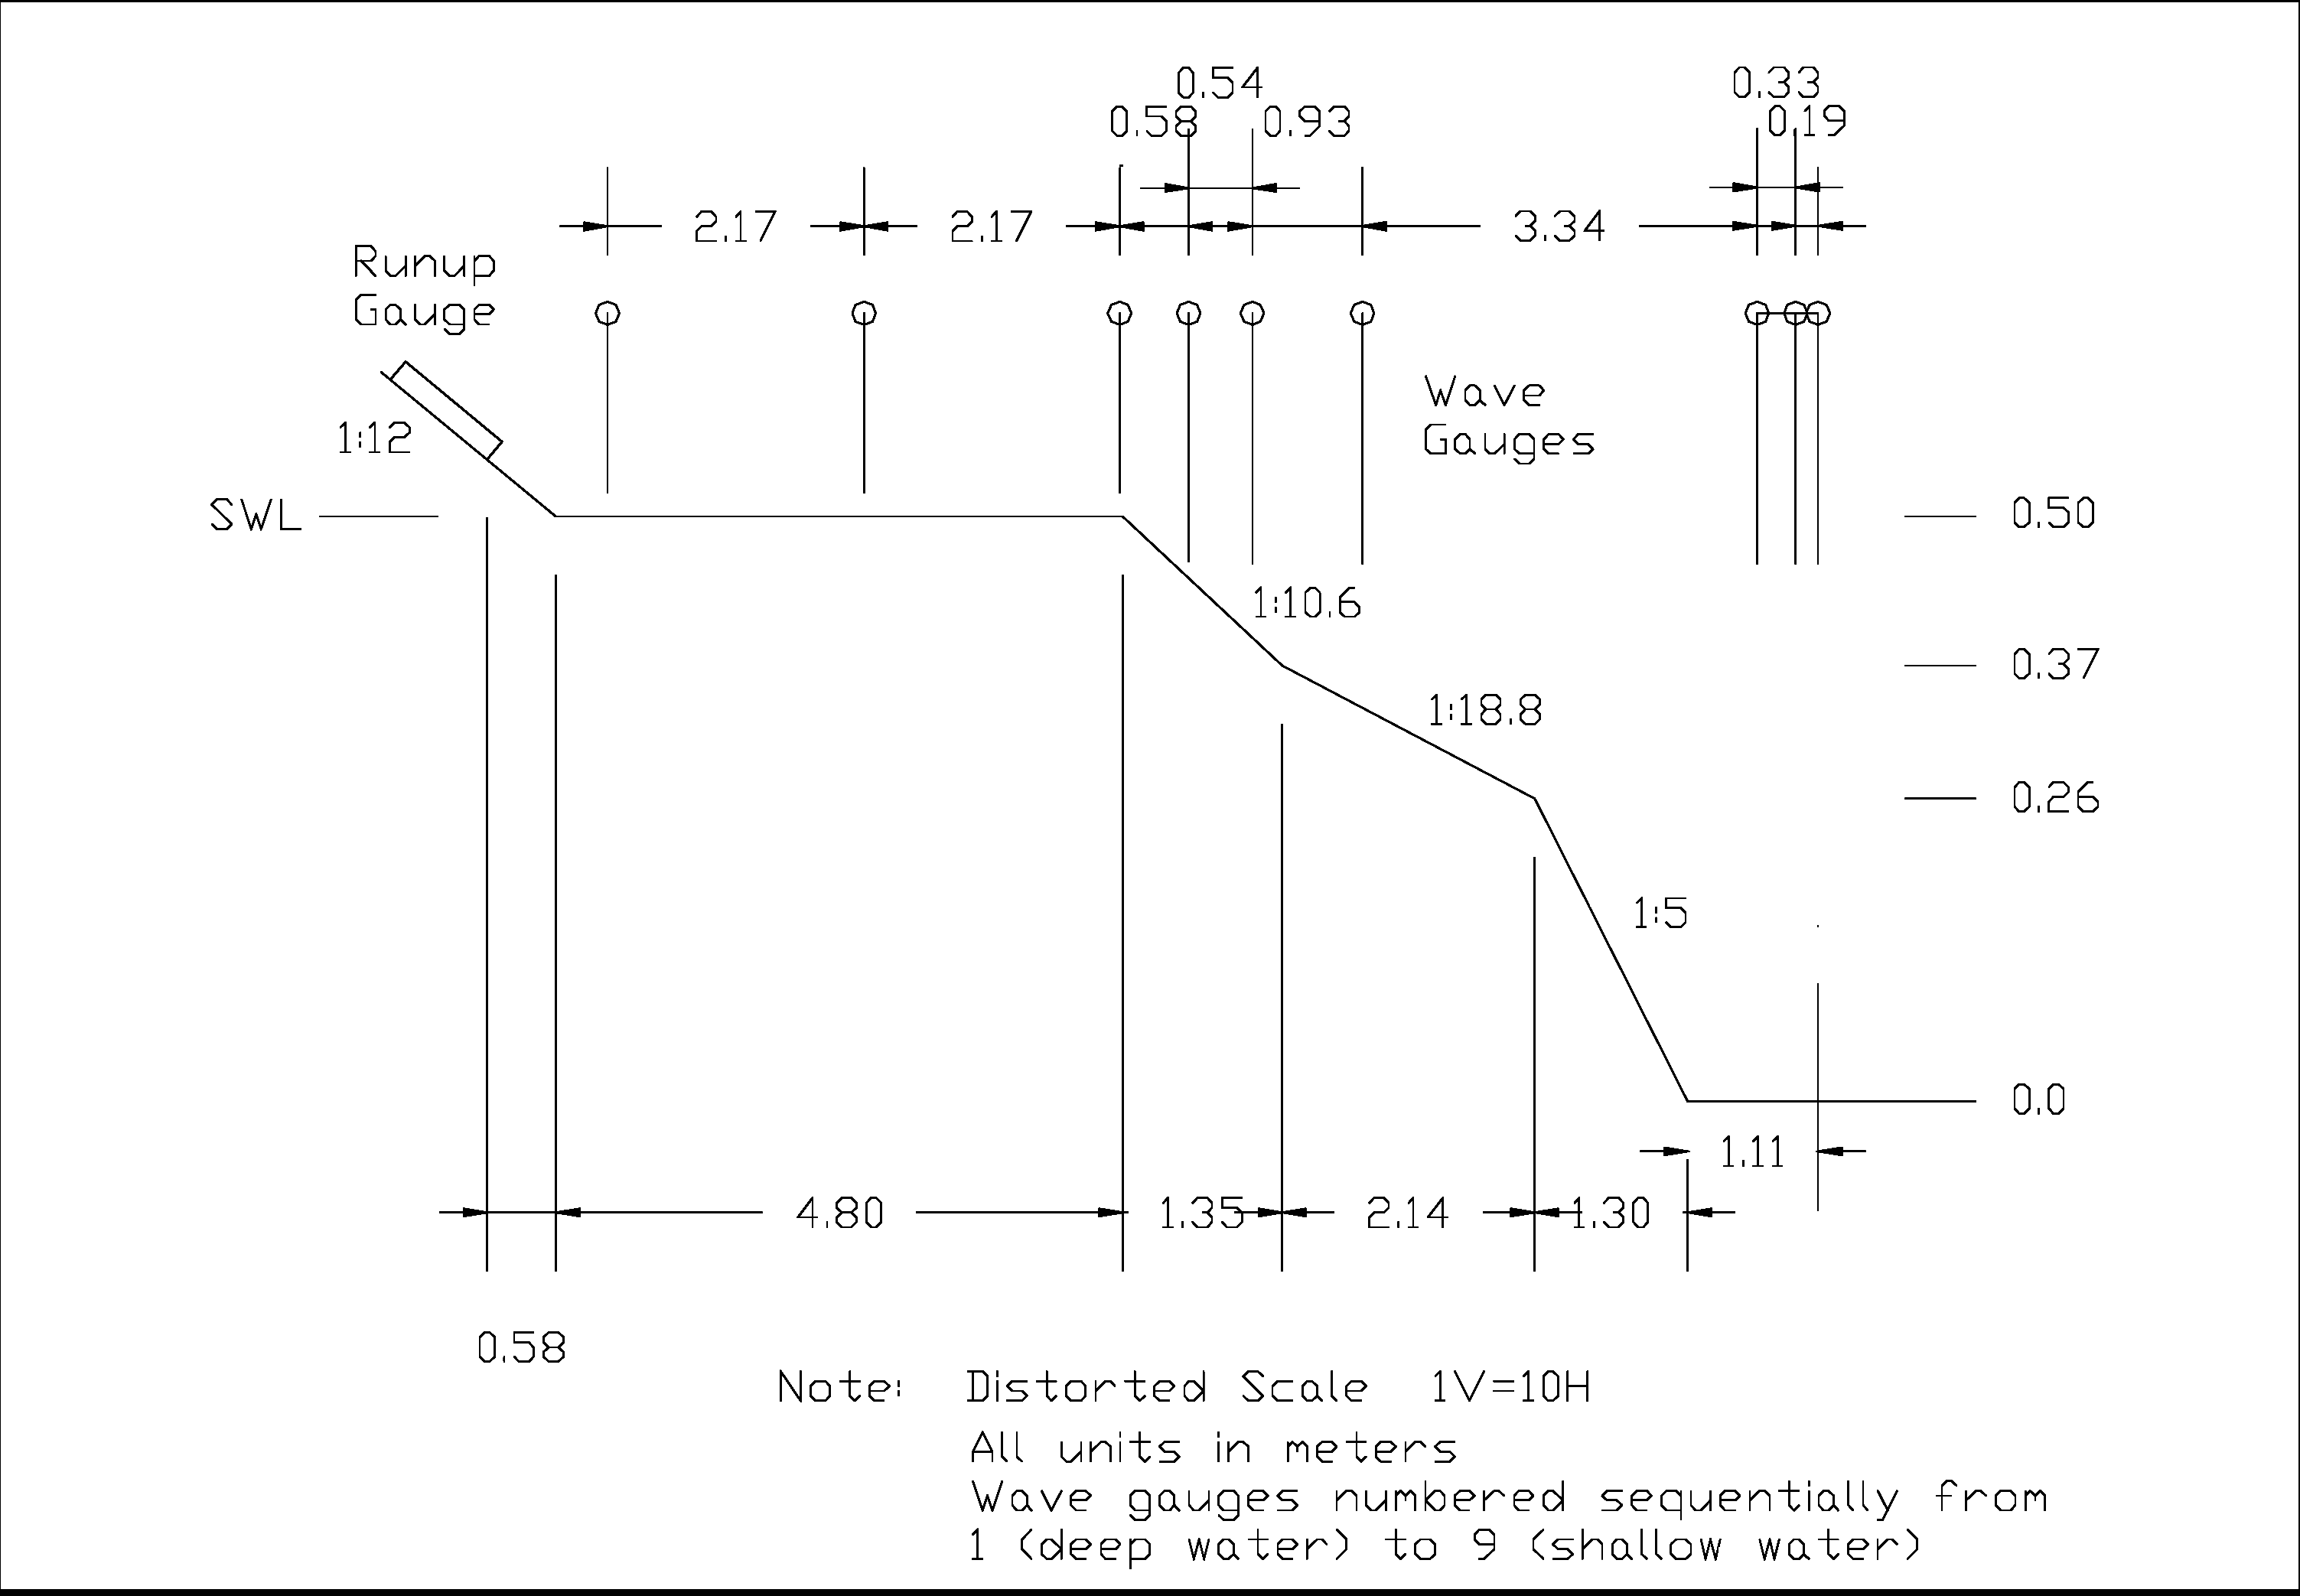
\includegraphics[scale=0.2]{./images/instrumen_eksperimen.png}
  \end{center}
  \caption{}
\end{figure}
\FloatBarrier

Pada eksperimen ini ada 9 sensor gelombang, 2 sensor kecepatan angin, dan 1 sensor \emph{runup} gelombang. Wilayah penyebaran sensor gelombang dikelompokan menjadi 2. Wilayah pertama berada di atas karang dan wilayah kedua berada di laut.. Wilayah karang merupakan gabungan dari wilayah karang yang datar \emph{Reef Flat} dan wilayah karang yang miring. Wilayah karang datar memiliki panjang mulai dari \emph{SWL} hingga 4.8 meter ke arah laut. Wilayah karang yang miring \emph{Reef Slope} di mulai dari bibir karang datar hingga 4.79 meter ke arah laut. Laut didefinisikan dengan wilayah dengan dasar terdalam. Untuk sensor 1, 2, dan 3 tersebar di wilayah laut, sensor 4, 5, dan 6 tersebar di wilayah \emph{reef slope}, dan untuk sensor 7, 8, dan 9 tersebar di wilayah \emph{reef flat}.

\pagebreak

\subsection{Hasil Analisa Data}

Dari laporan \emph{"Laboratory Study of Wind Effect on Runup over Fringing Reefs"} \cite{DemirbilekReport} data yang di hasilkan berupa data hasil analisa yang berasal dari raw data yang merupakan time series. Pada table tersebut $H$ merupakan tinggi gelombang, $T$ merupakan spectral peak periods, $WL$ merupakan Wave Length, dan $R_{max}$ adalah ketinggian maksimum dari \emph{runup}. $H$, $WL$, dan $R_{max}$ merupakan dalam $cm$.

\begin{table}
    \begin{center}
      \begin{tabular}{|l|l|l|l|l|l|l|l|}
      \hline
      TestId & H & T & WL & $R_{max}$ & Wind \\ \hline
      Test99 & 5.5 & 1.25 & 50.0 & 1.5 & 7.1 \\ \hline
      Test100 & 6.0 & 1.0 & 50.0 & 1.6 & 6.9 \\ \hline
      Test101 & 3.3 & 1.0 & 50.0 & 0.7 & 5.3 \\ \hline
      Test102 & 8.2 & 2.5 & 53.1 & 8.4 & 7.0 \\ \hline
      Test103 & 8.6 & 2.0 & 53.1 & 7.8 & 7.1 \\ \hline
      Test104 & 8.0 & 1.75 & 53.1 & 6.7 & 5.8 \\ \hline
      Test105 & 7.8 & 1.5 & 53.1 & 5.9 & 6.3 \\ \hline
      Test106 & 5.4 & 1.5 & 53.1 & 4.0 & 6.7 \\ \hline
      Test107 & 6.3 & 1.25 & 53.1 & 4.5 & 6.8 \\ \hline
      Test108 & 6.6 & 1.0 & 53.1 & 6.4 & 6.7 \\ \hline
      Test109 & 3.8 & 1.0 & 53.1 & 5.3 & 6.5 \\ \hline
      \end{tabular}
    \end{center}
    \caption{Sampel data hasil analisa.}
  \end{table}
\FloatBarrier

\section{Model Artificial Neural Network}
  Pada TA ini, digunakan model ANN dengan 1 hidden layer (\emph{Non-deep Neural Network}). Terdapat 4 input, yang berupa vector dengan masing-masing nilai berupa $H$ (\emph{Significant Height} Gelombang) dalam $cm$, $T$ (\emph{Spectral Peak Periods}) dalam $detik$, $WL$ (\emph{Wave Length}) dalam $cm$, dan $WIND$ (kecepatan angin) dalam $meter/detik$. Model AAN ini memiliki 1 output dan merupakan model \emph{regressi linear}. Output merupakan prediksi ketinggian \emph{runup} dengan satuan $cm$.

  \def\layersep{4cm}
  \begin{figure}
    \begin{tikzpicture}[shorten >=1pt,->,draw=black!50, node distance=\layersep]
        \tikzstyle{every pin edge}=[<-,shorten <=1pt]
        \tikzstyle{neuron}=[circle, fill=black!25,minimum size=17pt,inner sep=0pt]
        \tikzstyle{input neuron}=[neuron, fill=green!50];
        \tikzstyle{output neuron}=[neuron, fill=red!50];
        \tikzstyle{hidden neuron}=[neuron, fill=blue!50];
        \tikzstyle{annot} = [text width=4em, text centered]

        % Draw the input layer nodes
        \node[input neuron, pin=left:H] (I-H) at (0,-1) {};
        \node[input neuron, pin=left:WL] (I-T) at (0,-2) {};
        \node[input neuron, pin=left:WIND] (I-WL) at (0,-3) {};
        \node[input neuron, pin=left:T] (I-WIND) at (0,-4) {};

        % Draw the hidden layer nodes
        \path[yshift=0.0cm]{}
            node[hidden neuron] (H-1) at (\layersep,-1 cm) {};
        \path[yshift=0.0cm]{}
            node[hidden neuron] (H-2) at (\layersep,-2 cm) {};
        \path[yshift=0.0cm]{}
            node[hidden neuron] (H-3) at (\layersep,-3 cm) {};
        \path[yshift=0.0cm]{}
            node[hidden neuron] (H-4) at (\layersep,-4 cm) {};

        % Draw the output layer node
        \node[output neuron,pin={[pin edge={->}]right:Prediksi Runup}, right of=H-3] (O) {};

        % Connect every node in the input layer with every node in the
        % hidden layer.
        \foreach \source in {H, T, WL, WIND}
            \foreach \dest in {1,...,4}
                \path (I-\source) edge node[midway, right] {$W_{hidden}$} (H-\dest);

        % Connect every node in the hidden layer with the output layer
        \foreach \source in {1,...,4}
            \path (H-\source) edge node[midway, right] {$W_{output}$} (O);

        % Annotate the layers
        \node[annot,above of=H-1, node distance=1cm] (hl) {Hidden layer};
        \node[annot,left of=hl] {Input layer};
        \node[annot,right of=hl] {Output layer};
        \label{modelANNTA}
    \end{tikzpicture}
    \caption{Model ANN yang digunakan pada TA ini.}
  \end{figure}
  \FloatBarrier

\section{Flowchart Sistem TA}

Secara keseluruhan, terdapat bentuk hirarki dalam sistem ini. Hirarki \emph{root} (Hirarki Utama), yakni sistem itu sendiri, bertugas sebagai pengatur. \emph{Root} memiliki anak yang memiliki tugas-tugas tertentu, seperti: \emph{Membaca File}, \emph{Transformasi Data}, \emph{Membagi Data}, atau yang paling penting yakni \emph{Training Data}.

\subsection{Flowchart Sistem Utama}

  Sistem utama merupakan pengatur dari komponen-komponen yang ada pada sistem TA ini. Komponen-komponen tersebut termasuk: Pembacaan Data, Transformasi Data, Pembagian Data, Inisialisasi Epoch Dan Learning Rate, Melakukan Training, dan Melakukan Testing.

  Sistem dimulai dengan membaca data. Pembacaan data dibagi menjadi 2. Pembacaan data training dan pembacaan data testing. Data training mencakup 80 persen dari seluruh data observasi, sedangkan data training mencakup 20 persen. Hal ini sejalan dengan Fan et al \cite{fan2008liblinear}, dimana beliau menggunakan rasio 80/20 untuk training dan testing. Setelah melakukan pembacaan data, sistem akan melakukan transformasi data. Mengubah data csv, menjadi matriks dengan panjang kolom 4, yang mewakili $H$, $T$, $WL$, dan $WIND$. Komponen selanjutnya adalah inisialisasi \emph{epoch} dan \emph{learning rate}. \emph{Epoch} adalah representasi dari keseluruhan data yang digunakan pada training. Sedangkan \emph{learning rate} adalah besaran dari suatu langkah pembelajaran. Nilai dari \emph{learning rate} dan \emph{epoch} selanjutnya akan dimasukan ke dalam fungsi training. 

\begin{figure}[ht]
  \caption{Flowchart Sistem Utama}
  \begin{center}
    \tikzstyle{decision} = [diamond, draw, 
        text width=4.5em, text badly centered, node distance=3cm, inner sep=0pt]
    \tikzstyle{block} = [rectangle, draw, 
        text width=12em, text centered, minimum height=2em]
    \tikzstyle{circle} = [draw, ellipse, minimum height=2em, distance=4em]
    \tikzstyle{blockTraining} = [rectangle, draw, fill=red!20, 
        text width=12em, text centered, minimum height=2em]
    \tikzstyle{line} = [draw, -latex']
        
    \begin{tikzpicture}[node distance = 2.3cm, auto]
        % Place nodes
        \node [circle] (init) {Mulai};
        \node [block, below of=init] (bacaData) {Membaca data report dari csv file};
        \node [block, below of=bacaData] (transformasiData) {Transformasi data menjadi matrix};
        \node [block, below of=transformasiData] (setupEpochLr) {Menentukan jumlah epoch dan learning rate};
        \node [blockTraining, below of=setupEpochLr] (training) {Melakukan Training};
        \node [blockTraining, below of=training] (testing) {Melakukan Testing};
        \node [circle, below of=testing] (stop) {Stop};
      
        % Draw edges
        \path [line] (init) -- (bacaData);
        \path [line] (bacaData) -- (transformasiData);
        \path [line] (transformasiData) -- (setupEpochLr);
        \path [line] (setupEpochLr) -- (training);
        \path [line] (training) -- (testing);
        \path [line] (testing) -- (stop);
        \label{fig:sistem}
    \end{tikzpicture}
  \end{center}
\end{figure}
\FloatBarrier

\subsection{Flowchart Komponen Training Dan Testing}
\label{FlowChartTraining}
Pada bagian training dan testing \ref{fig:sistem}, algoritma yang digunakan adalah algoritma ANN. Untuk testing, hanya dilakukan algoritma \emph{Feed Forward}.

Algoritma ANN dimulai dengan inisialisasi weight dengan random data. Selanjutnya, nilai pada \emph{input parameter} akan dikalikan dengan $weight$ \emph{hidden layer} $W^1$, sehingga dihasilkan $a^1$. Untuk menjadi nilai pada \emph{neuron hidden layer} $z^1$, $a$ akan diaktifasi dengan fungsi aktivasi $RELU$ sehingga nilai $z^1$ merupakan hasil dari $relu(a)$. Untuk mengahasilkan nilai prediksi, $z^1$ dikalikan dengan $weight$ pada \emph{output} $W^2$, sehingga mengasilkan $a^2$. Nilai $a^2$ merupakan nilai hasil prediksi, karna fungsi aktivasi dari \emph{output} adalah linear ($f(a) = a$).

\begin{figure}[ht]
  \caption{Flowchart Komponen Training Dan Testing}
  \begin{center}
    \tikzstyle{block} = [rectangle, draw, fill=blue!20, 
        text width=10em, text centered, minimum height=6em]
    \tikzstyle{blockTraining} = [rectangle, draw, fill=red!20, 
        text width=14em, text centered, minimum height=2em]
    \tikzstyle{stopTrainng} = [rectangle, draw, fill=red!20, 
        text width=3em, text centered,  distance=10cm]
    \tikzstyle{line} = [draw, -latex']
    \tikzstyle{circle} = [draw, ellipse, minimum height=2em, distance=4em]
    \tikzstyle{decision} = [diamond, draw, fill=blue!20, 
        text width=4em, text badly centered, node distance=2.5cm, inner sep=0pt]
        
    \begin{tikzpicture}[node distance = 2cm, auto]
        % Place nodes
        \node [circle] (init) {Mulai};
        \node [blockTraining, below of=init] (randomWeight) {Inisialisasi $weight$ dengan random data};
        \node [blockTraining, below of=randomWeight] (IW){Mengalikan Input Layer Dengan $Weight$ hidden layer};
        \node [blockTraining, below of=IW] (aktivasi){Jalankan fungsi aktivasi hidden layer};
        \node [blockTraining, below of=aktivasi] (HW){Mengalikan Input Layer Dengan $Weight$ untuk $output$};
        \node [blockTraining, below of=HW] (aktivasiOutput){Menjalankan fungsi aktivasi untuk output neuron};
        \node [blockTraining, below of=aktivasiOutput] (cost){Kalkulasi Error};
        \node [circle, below of=cost] (stop){Stop};
  
        % Draw edges
        \path [line] (init) -- (randomWeight);
        \path [line] (randomWeight) -- (IW);
        \path [line] (IW) -- (aktivasi);
        \path [line] (aktivasi) -- (HW);
        \path [line] (HW) -- (aktivasiOutput);
        \path [line] (aktivasiOutput) -- (cost);
        \path [line] (cost) -- (stop);
    \end{tikzpicture}
  \end{center}
\end{figure}
\FloatBarrier

%
\chapter{Preliminary Results}
Berikut adalah preliminary result dari ``{\Title}''. Data yang digunakan dalam preliminary result ini adalah data yang berasal dari data \emph{testing}. Yakni, 8 data, yang merepresentasikan 20 persen dari keseluruhan data hasil  observasi.

\begin{figure}[ht]
  \begin{center}
    \begin{tikzpicture}
      \begin{axis}[
        xlabel=Nomor Data,
        ylabel=Tinggi Runup]
      \addplot table [y=predicted, x=num]{relu_10000.dat};
      \addlegendentry{$Hasil Prediksi$}
      \addplot table [y=measured, x=num]{relu_10000.dat};
      \addlegendentry{$Hasil Observasi$}
      \end{axis}
    \end{tikzpicture}
    \caption{Hasil Prediksi Dengan Menggunakan Neural Network}
  \end{center}
\end{figure}

Berdasarkan running data test terhadap model yang diproduksi saat \emph{training}, data hasil prediksi memiliki Mean Square Error sebesar $2.07902920991855$. Dari 8 data prediksi, terdapat 5 data dengan Square Error dibawah 1.

%

%%%%%%%%%%%%%%%%%%%%%%%%%%%%%%%%%%%%%%%%%%%%%%%%%%%%%%%%%%%%%%%
% Berikut adalah untuk membuat Daftar pustaka
% Style daftar pustaka dapat disesuaikan dengan mengubah 
%\bibliographystyle{kode}
% dengan kode = acm maka hasinya contoh [1]
% dengan kode = agsm maka hasilnya Harvard style (Sukimin, 2017)
%%%%%%%%%%%%%%%%%%%%%%%%%%%%%%%%%%%%%%%%%%%%%%%%%%%%%%%%%%%%%%%%
\cleardoublepage
\addcontentsline{toc}{chapter}{Daftar Pustaka}
\bibliographystyle{plain} %harvard style
\bibliography{References.bib}
%
%\pagebreak
%%%%%%%%%%%%%%%%%%%%%%%%%%%%%%%%%%%%%%%%%%%%%%%%%%%%%%%%%%%%%%%
% Berikut untuk lampiran
%%%%%%%%%%%%%%%%%%%%%%%%%%%%%%%%%%%%%%%%%%%%%%%%%%%%%%%%%%%%%%
\cleardoublepage
\addcontentsline{toc}{chapter}{Lampiran}
\chapter*{Lampiran}

\end{document}
